\section{User-Interface}

Für die Umsetzung des UI wurde das \enquote{Bootstrap} CSS-Framework verwendet. Ausserdem wurden alle
HTML-Templates in der Ruby SLIM templating-language geschrieben, 
welche eine stark vereinfachte Syntax ohne \enquote{Brackets} und ohne \enquote{Closing-Tags} bietet.

Durch diese zwei Mittel und mit der Hilfe der in der Planungsphase erstellten Mockups \ref{}, konnte das UI
rasch umgesetzt werden und ist durch eine klare farbliche Hierarchie ergonomisch strukturiert. Wo nötig, wurden auch
Icons eingesetzt. 

\subsection{Assessments erstellen und verwalten}

\begin{figure}[H]
  \centering
  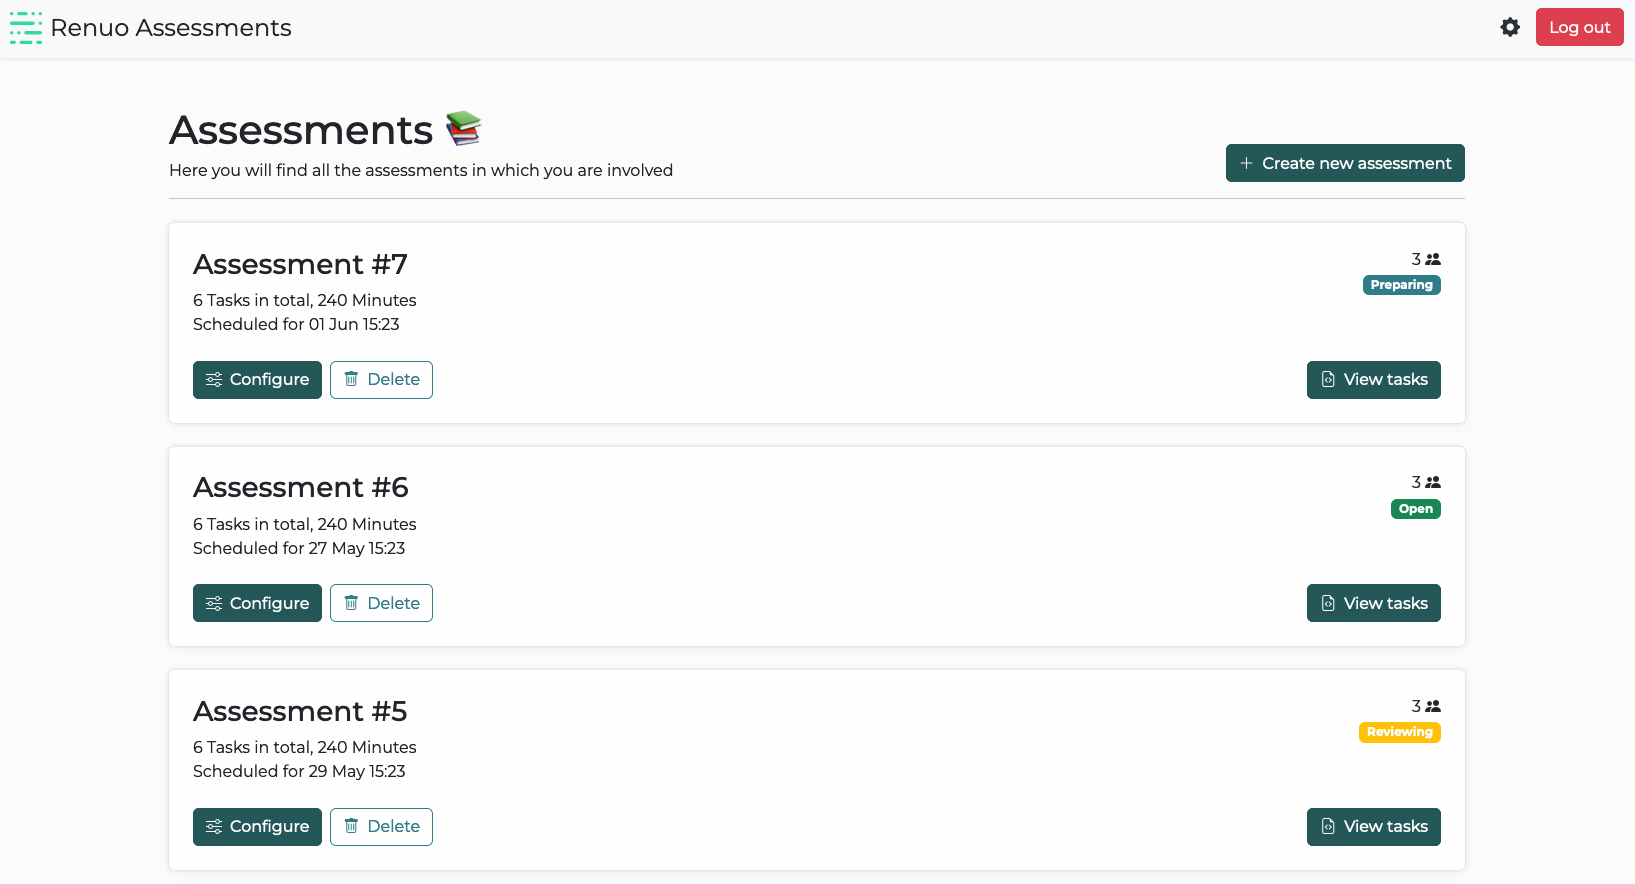
\includegraphics[width=\textwidth]{images/ui/assessments-index.png}
  \caption{\label{fig:assessments-index}Index-Seite, die alle Assessments auflistet}
\end{figure}

\begin{figure}[H]
  \centering
  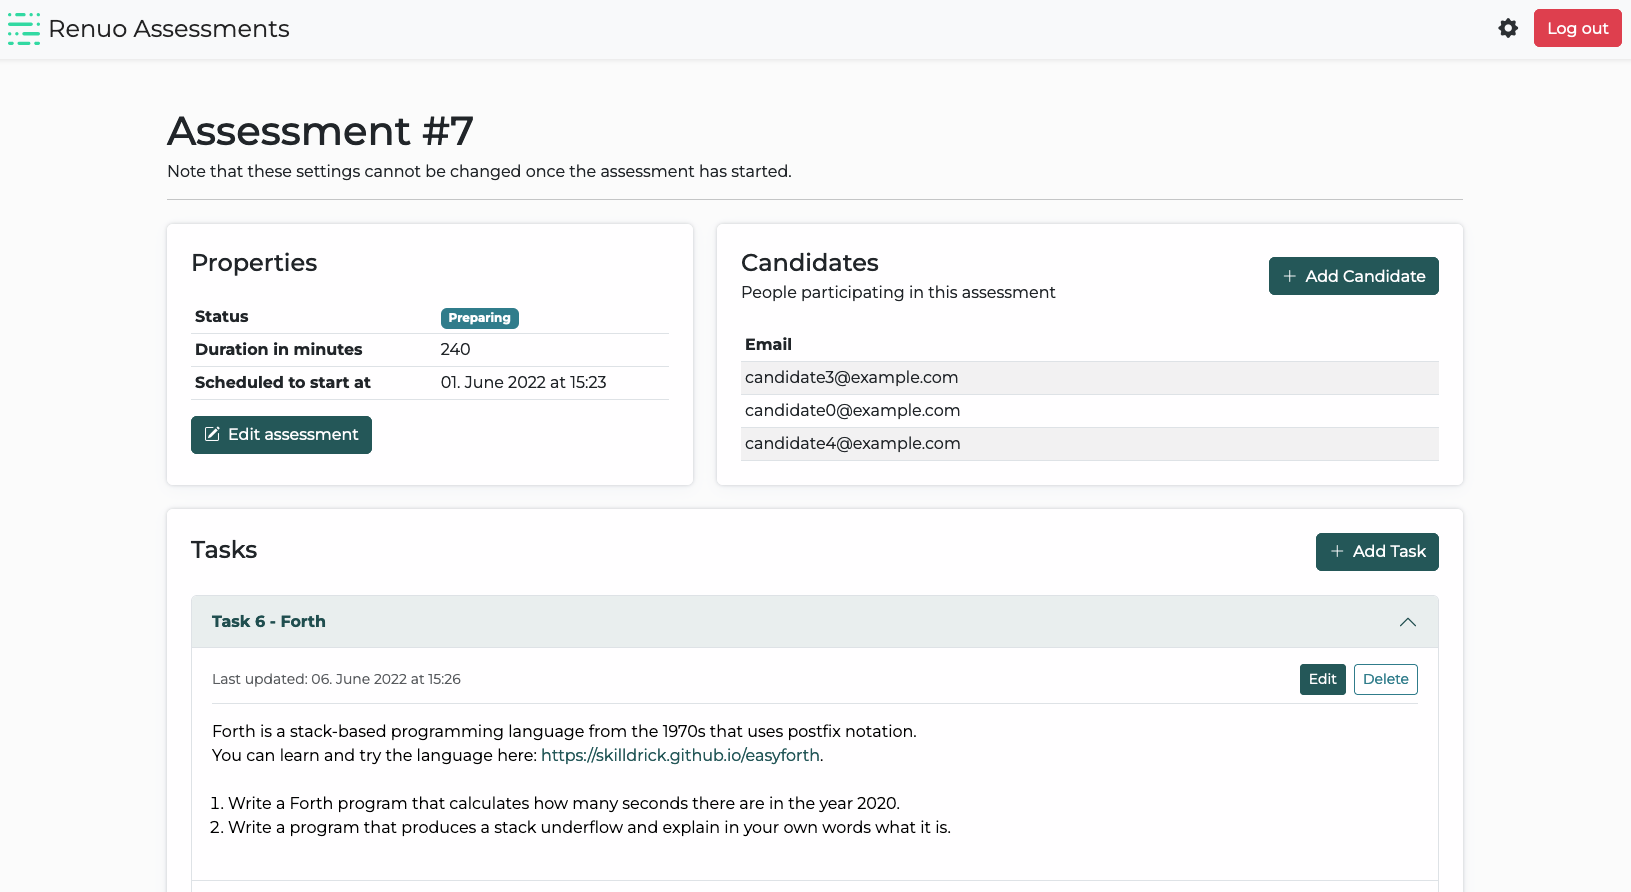
\includegraphics[width=\textwidth]{images/ui/assessments-edit.png}
  \caption{\label{fig:assessments-edit}Konfiguration des Assessments}
\end{figure}

\subsection{Assessments lösen}

\begin{figure}[H]
  \centering
  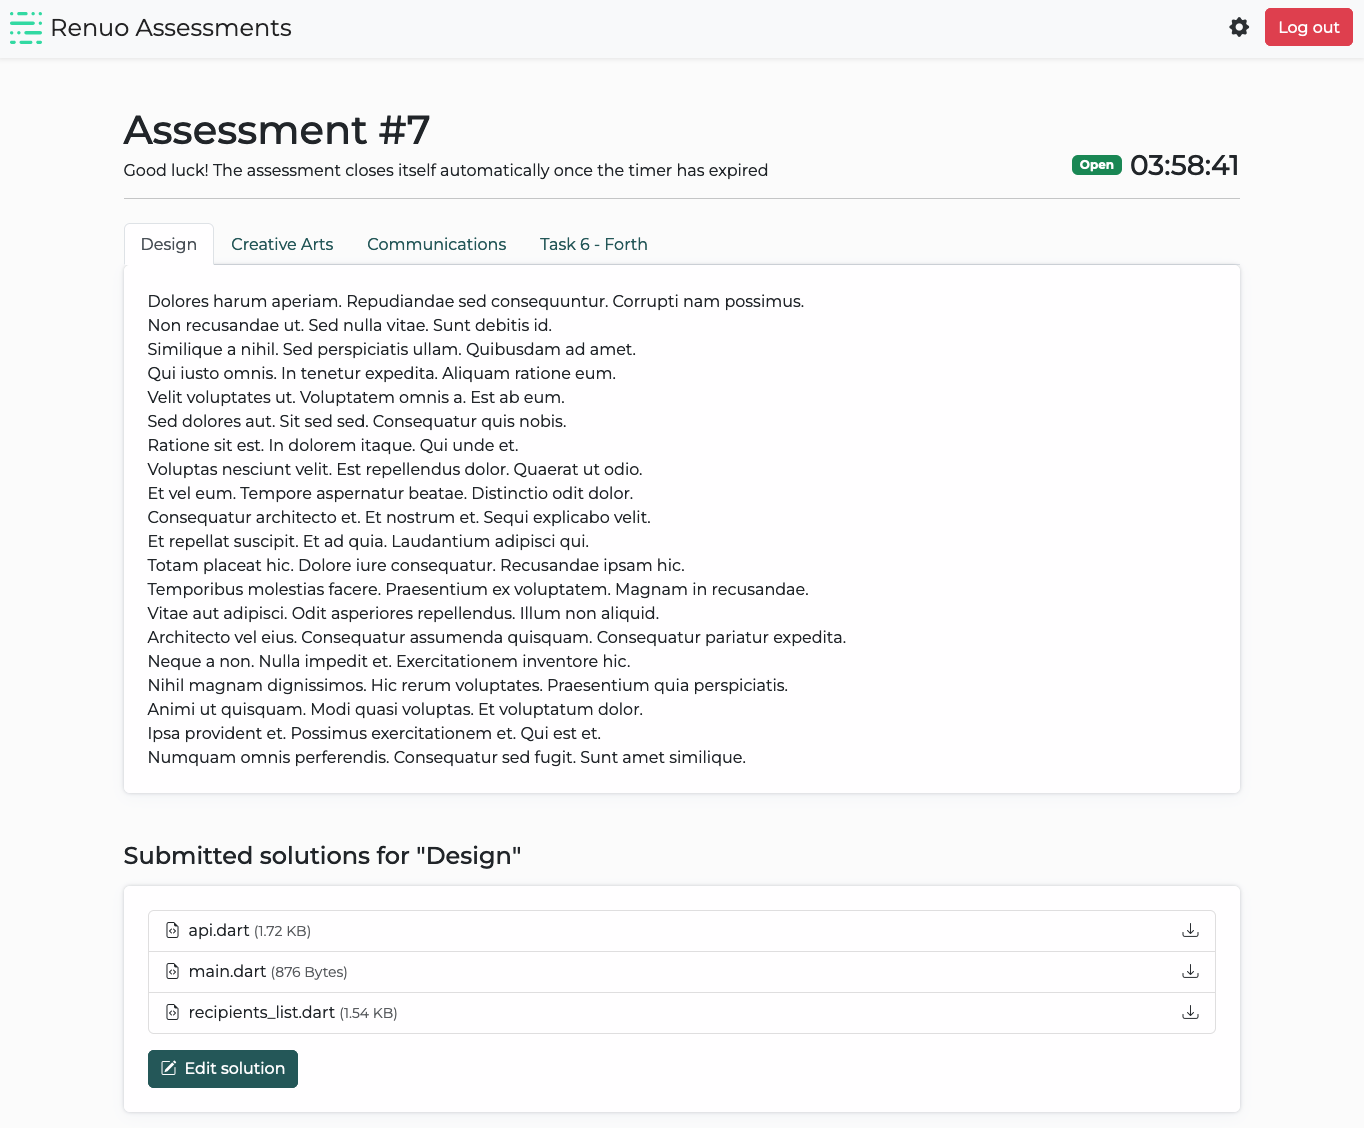
\includegraphics[width=14cm]{images/ui/solve-assessment.png}
  \caption{\label{fig:solve-assessment}Lösen eines Assessments}
\end{figure}


\subsection{Assessments korrigieren}

\begin{figure}[H]
  \centering
  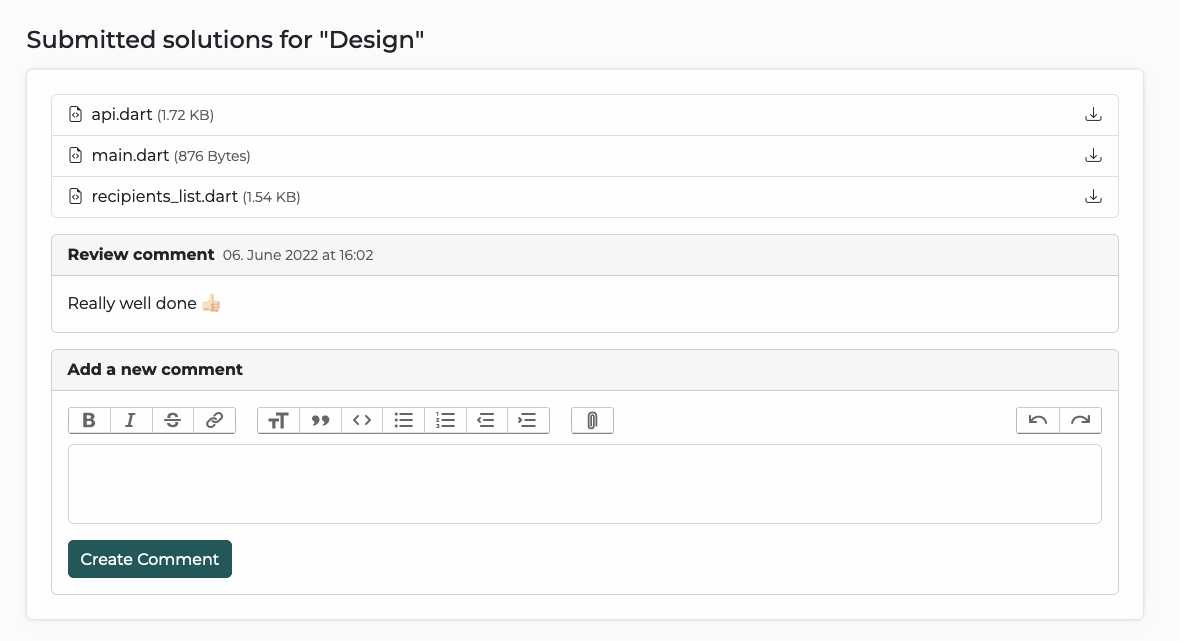
\includegraphics[width=14cm]{images/ui/review-comments.png}
  \caption{\label{fig:review-comments}Assessment auswerten}
\end{figure}
